\section{Anforderungsbeschreibung}
\textbf{Sicherheitsrelevanz, Diedienen, Beobachten, Anbringungspunkte von Bauteilen --> gefedert? --> Bahntauglichkeit}
Anhand des Ist- und Soll-Zustandes sind fünf Ausbaustufen für den Güterwagen 4.0 geplant. Hier eine Kurzbeschreibung der geplanten Ausbaustufen:\par
\textbf{Ausbaustufe 1: Stromversorgung, Telematik und Datenvernetzung}\par
\begin{figure}[hbp] 
    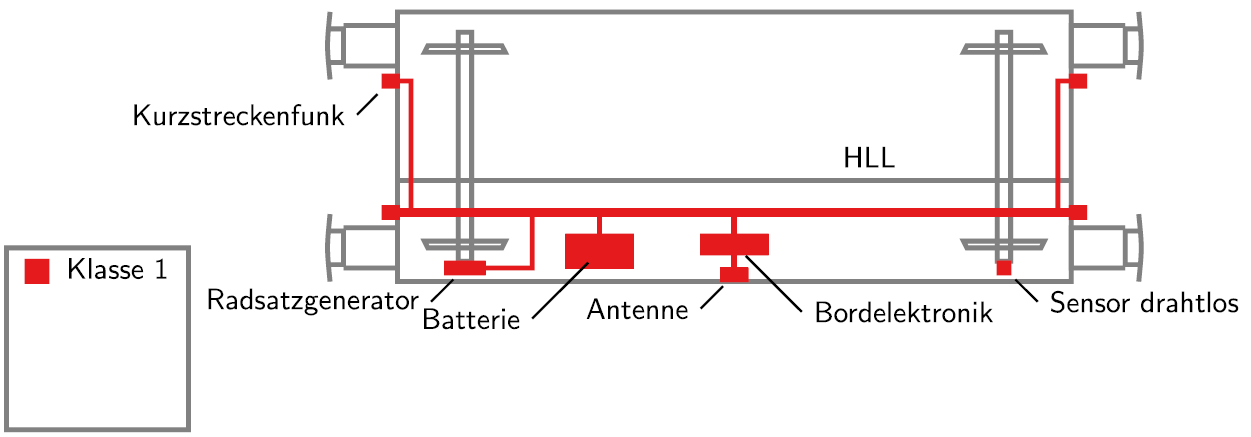
\includegraphics[width=\textwidth]{Bilder/Ausbaustufen_1.PNG}
    \caption{Klasse 1 mit Stromversorgung, Telematik und Datenvernetzung - angelehnt an \cite{Ausbaustufen} }
    \label{fig:Klasse1}
\end{figure} 
In der ersten Ausbaustufe, siehe Abbildung \ref{fig:Klasse1}, ist geplant Bordelektronik und eine entsprechende Spannungsversorgung anzubringen. Diese kann als Batterie mit Speisung durch einen Radsatzgenerator, Solarpanels oder ähnlichem realisiert werden oder auch als Pufferbatterie mit Speisung durch AK. Dazu kommen verschiedene Antennen und Kurzstreckenfunk zur Kommunikation mit anderen Wagen. Auch Sensoren zur Erfassung verschiedener Telematikfunktionen sind geplant.\par
In diesem Stadium ist der Wagen an sich noch nicht 'schlauer' als ein nicht ausgerüsteter Wagen, aber er kann sich mitteilen. Mitteilungen könne sein: Standort, Belandung, Laufleistung, (ungewöhnliche) Vibrationen (beispielsweise durch Falschstellen), Heißläuferdedektion, letzte Wartungsintervalle, Zustand der Bremse und vieles mehr.\par
\textbf{Ausbaustufe 2: Ausbaustufe 1 + Automatisierung der Bremsbedienung}\par
\begin{figure}[htbp] 
    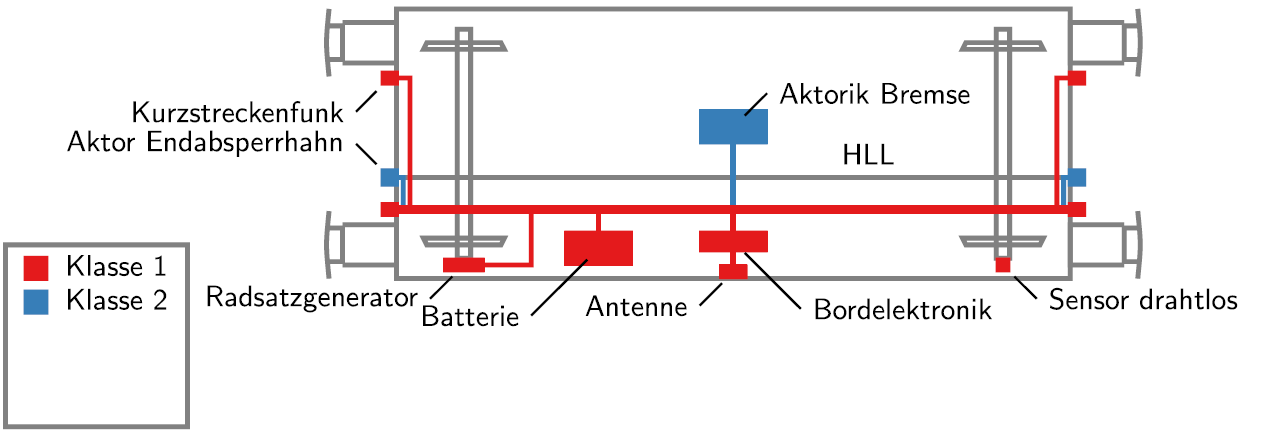
\includegraphics[width=\textwidth]{Bilder/Ausbaustufen_2.PNG}
    \caption{Klasse 2 bestehend aus Klasse 1 und der Automatisierung der Bremsbedienung - angelehnt an \cite{Ausbaustufen}}
    \label{fig:Klasse2}
\end{figure} 
In der zweiten Ausbaustufe ist eine zusätzliche Aktorik für Endabsperrhähne und Handbremse geplant. Dadurch kann ein Teil der Bremsbedienung sow weit automatisiert werden, dass ein Einstellen der Bremsart anhand von anderen Wagen im Wagenzug, Gewicht und Bremsfähigkeit möglich ist. Außerdem ist die automatische Parkbremse realisiert.\par
\textbf{Ausbaustufe 3: Ausbaustufe 2 + ep-''light''-Bremsen}\par
\begin{figure}[htbp] 
    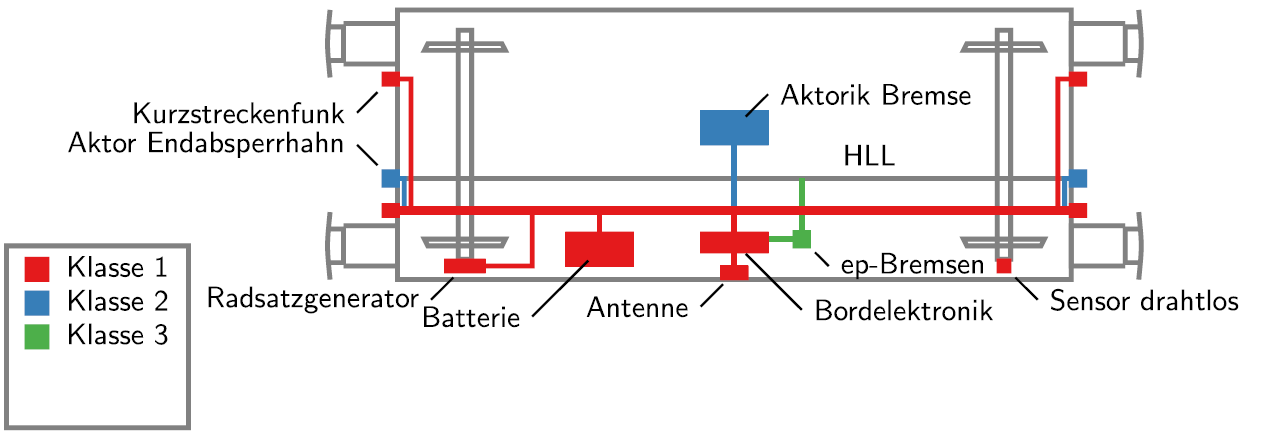
\includegraphics[width=\textwidth]{Bilder/Ausbaustufen_3.PNG}
    \caption{Klasse 3 bestehend aus Klasse 2 und der eingeführten ep-''light'-Bremse - angelehnt an \cite{Ausbaustufen}}
    \label{fig:Klasse3}
\end{figure} 
In der dritten Ausbaustufe kommt zusätzlich zur Bremsbedienung auch die Ep-''light''-Bremse hinzu. Diese sorgt für eine für kürzere Bremswege und/oder höhere Geschwindigkeiten.\par
\textbf{Ausbaustufe 4: Ausbaustufe 3 + automatisierter Zugschluss}\par
\begin{figure}[htbp] 
    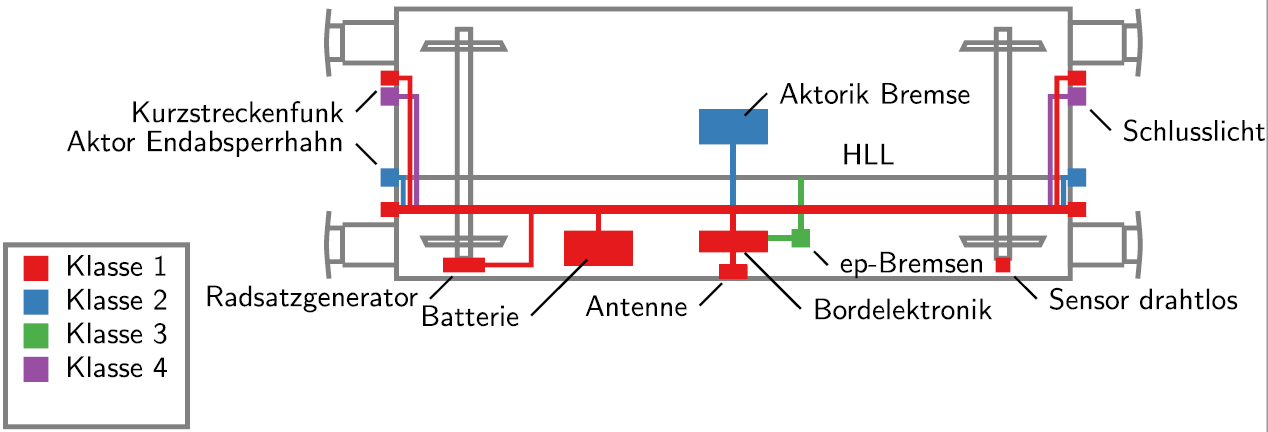
\includegraphics[width=\textwidth]{Bilder/Ausbaustufen_4.PNG}
    \caption{Klasse 4 bestehend aus Klasse 3 und der Automatisierung des Zugschlusses - angelehnt an \cite{Ausbaustufen}}
    \label{fig:Klasse4}
\end{figure} 
In der vierten Ausbaustufe ist ein automatisierter Zugschluss geplant, neben der dann noch lästigen Aufgabe den kompletten Wagenzug langzulaufen um am letzen Wagen ein Zugschluss-Signal zu stecken soll mit dieser Funktion auch die Zugintigrität gewährleistet werden.\par
\textbf{Ausbaustufe 5: Ausbaustufe 4 + Rangierantrieb}\par
\begin{figure}[htbp] 
    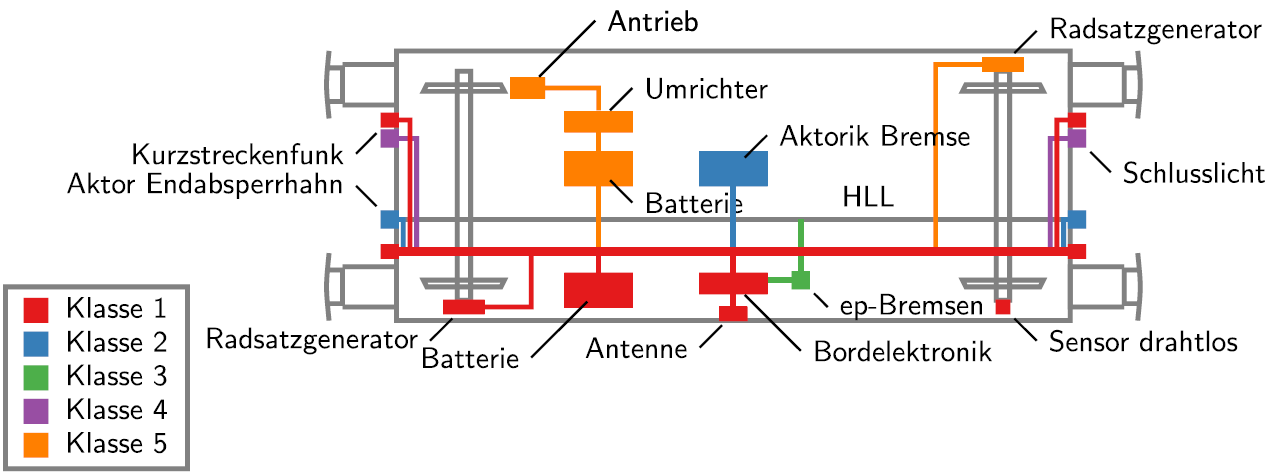
\includegraphics[width=\textwidth]{Bilder/Ausbaustufen_5.PNG}
    \caption{Klasse 5 bestehend aus Klasse 4 und einem Rangierantrieb - angelehnt an \cite{Ausbaustufen}}
    \label{fig:Klasse5}
\end{figure} 
In der fünften Ausbaustufe kommt der Rangierantrieb hinzu. Damit dieser ohne Probleme funktioniert brauch er er zusätzlich eine weitere Batterie und Umrichter. Zur Speisung der zweiten Batterie wird auch ein zweiter Radsatzgenerator eingebaut.\par
In diesem Stadium kann von einem automatisierten Güterwagen gesprochen werden. Er kann selbstständig bei der Briefkastenbedienung assistieren und auf dem Werksgelände ohne Rangierlok verfahren.\par
Die ersten drei Ausbaustufen sollen in diesem Projekt stattfinden. Ausbaustufe 4 und 5 in Folgeprojekten. Eine Zulassung soll über mindestens gleichbleibende Sicherheit bei kompletter Abschaltung des Systems stattfinden. Diese in Schritten stattfindende Automatisierung führt zu einem hohen Mehrwert des Güterwagens, nicht nur, im Einzelwagenverkehr.
